\chapter{Evaluation}   \label{ch:6:eval}

In this section, the main body of work is evaluated based on objectives defined at the beginning of the project (Section \ref{objectives}) and are detailed as follows:
\begin{enumerate}
    \item Investigate the effect of different pre-processing techniques on semantic clustering and topic modelling.
    \item Investigate the effect of different word embedding models on the quality of clustering.
    \item Investigate the effect of different word embedding models and runtime environments on the performance (in terms of time efficiency).
    \item Evaluate the legibility of the results from the Topic Extraction Engine and Semantic Triple Extraction Engine based on user feedback.
\end{enumerate}

\section{Quantitative evaluation of semantic clustering} \label{s:evaluation_semantic_clustering}

\subsection{Effect of different processing techniques on clustering} \label{s:preprocess_clustering}

In order to cluster the news articles, different pre-processing techniques were applied to the article corpora in the topic extraction engine. The motivation behind this was to gauge the effect of these techniques on the silhouettes scores and incorporate the techniques that the result in the most optimal scores indicating improved clustering. As discussed in Section \ref{s:procesing_topic_engine}, the article corpora are pre-processed using techniques such as coreference resolution (CR), removing stopwords, removing named entities before obtaining article vectors for clustering. Figure \ref{fig:pre-processing_sil} illustrates how omitting these different pre-processing techniques affects the silhouette score of the semantic clustering obtained for the Year-Category data group: Travel 2021. We can see that not doing any pre-processing (`No pre-processing') on the articles in Travel 2021 data group results in a poor silhouette score of 0.36 compared to `All', which results in a silhouette score of 0.691 and involves performing coreference resolution, named entity removal and stopword removal. The silhouette score of 1 indicates dense, nicely separated clusters, a score of 0 indicates that clusters are overlapping, or distance between them is insignificant and -1 indicates incorrect clustering. Figure  \ref{fig:pre-processing_sil} shows that omitting these pre-processing techniques deteriorates the quality of clustering, by resulting in poor silhouette scores which indicate overlapping clusters.

\begin{figure}[H]
\centering
  \begin{minipage}[t]{.49\linewidth}
    \centering
    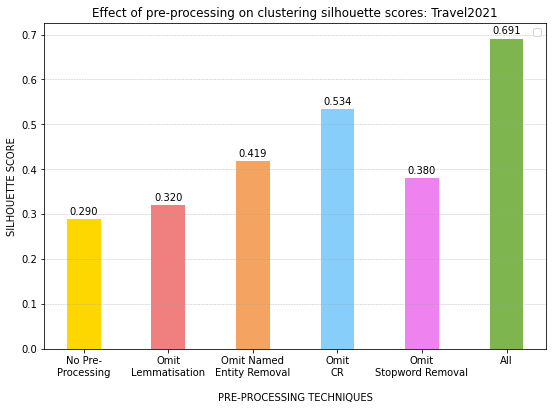
\includegraphics[width=\linewidth]{images/eval/effect_preprocessing.png}
    \caption{-}
    \label{fig:pre-processing_sil}
  \end{minipage}
  \begin{minipage}[t]{.49\textwidth}
    \centering
    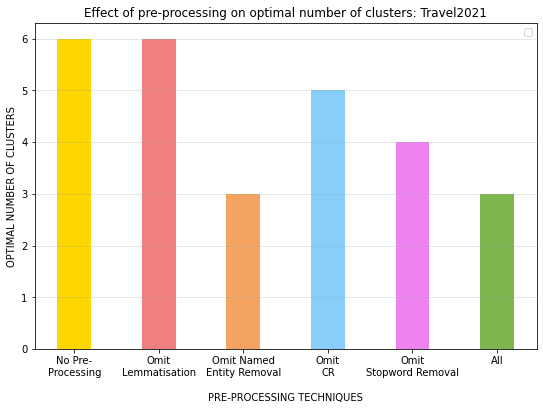
\includegraphics[width=\linewidth]{images/eval/preprocessing_cluster_no.png}
    \caption{-}
     \label{fig:pre-processing_cluster_no}
  \end{minipage}
\end{figure}

Another interesting takeaway is that post pre-processing considering the techniques in questions, usually results in lower number of clusters as seen in \Cref{fig:pre-processing_cluster_no}. Generally, the aim is to get the best silhouette score with smallest number of clusters. This is because the topic extraction engine should not try to over-cluster the data by fixating on small differences within the corpus. The semantic clusters are derived for topics to be modelled within them. In this example shown in the figure, Travel 2021 was selected as it has a very few number of member articles: 17. Not performing any pre-processing results in 6 clusters for a group of 17 articles. This is excessive as it means each semantic cluster has about 2 or 3 articles. Therefore, the topics extracted from these will be modelled on an extremely small corpus of about 2 articles. For the same data group, performing all the techniques mentioned, coreference resolution, named entity and stopword removal, results in a much smaller number of clusters: 3. In conclusion, the trend established by \Crefrange{fig:pre-processing_sil}{fig:pre-processing_cluster_no} is that performing the pre-processing techniques mentioned results in better silhouette scores with lower number of clusters, which indicates better clustering. 

% \todonum[inline]{Add LDA}

\subsection{Pre-processing: Filtering on POS tags} \label{s:pos_clustering}
% \todonum[inline]{And LDA}
Another key decision made to improve the clustering of the input data was to filter the tokens extracted from the articles by their Part-Of-Speech (POS) tags. The decision was made to use only nouns to the tokens that represent each article. \Crefrange{fig:pos_business2020}{fig:pos_pursuit2021} show the optimal cluster number and silhouette score for the Year-Category data groups: Business2020, Business2020, Politics2021 and Pursuit2021 when allowed POS tags are just `NOUN' and when they are `NOUN', `VERB', `ADJ' and `ADV'. These figures show the general trend is that having a noun only tokens list to represent the articles for generating article vectors for semantic clustering gives a higher silhouette score for a smaller number of clusters. For instance, in \Cref{fig:pos_business2021}, the silhouette score for noun only tokens list is 0.59 compared to 0.48 when tokens list contains nouns, adjectives, verbs and adverbs, resulting in a 23\% improvement in silhouette score and indicating better clustering for noun only tokens list. The same is true for \Crefrange{fig:pos_politics2021}{fig:pos_pursuit2021} which show an 8.3\% and 16.3\% improvement respectively for clustering articles based on noun only article corpus.

\begin{figure}[H]
\centering
  \begin{minipage}[t]{.49\linewidth}
    \centering
    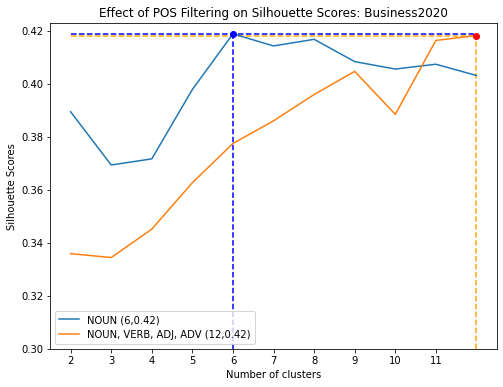
\includegraphics[width=\linewidth]{images/eval/business2020_sil.png}
    \caption{-}
    \label{fig:pos_business2020}
  \end{minipage}
  \begin{minipage}[t]{.49\textwidth}
    \centering
    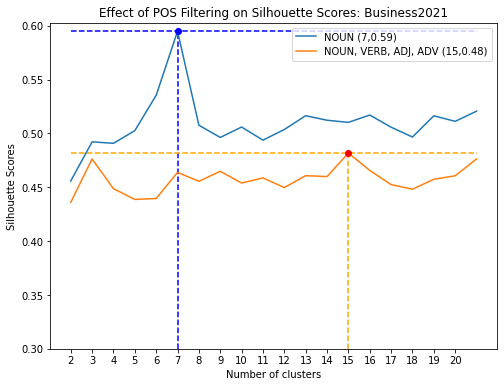
\includegraphics[width=\linewidth]{images/eval/business2021_sil.png}
    \caption{-}
    \label{fig:pos_business2021}
  \end{minipage}
  \begin{minipage}[t]{.49\textwidth}
    \centering
    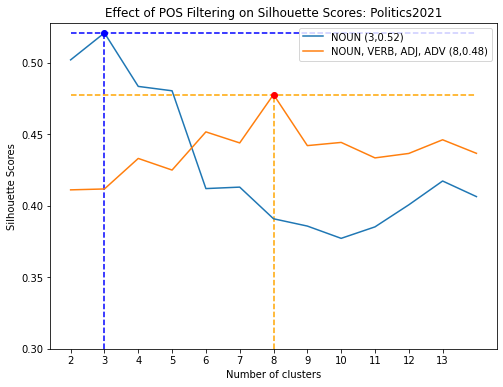
\includegraphics[width=\linewidth]{images/eval/politics2021_sil.png}
    \caption{-}
    \label{fig:pos_politics2021}
  \end{minipage}
  \begin{minipage}[t]{.49\textwidth}
    \centering
    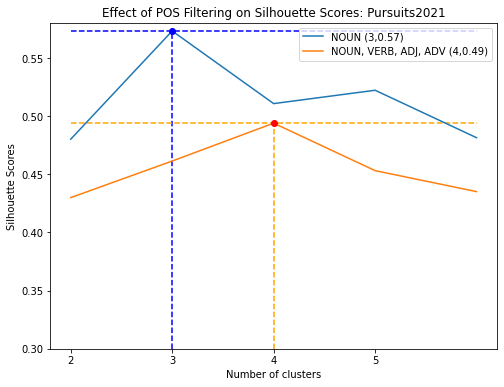
\includegraphics[width=\linewidth]{images/eval/pursuits2021_sil.png}
    \caption{-}
    \label{fig:pos_pursuit2021}
  \end{minipage}
\end{figure}

More evidently, it is important to note that the optimal number of clusters is much lower with a noun-only corpus as seen in the figures above. \Cref{fig:pos_business2020} shows that the silhouette score of 0.42 is achieved with only 6 clusters for noun-only tokens list compared to 12 with nouns, adjectives, verbs and adverbs. This makes sense as introducing adverbs, adjectives, verbs to the tokens list means that the article vectors will account for these tokens and result in a higher variance in the article vectors, making the corpus more difficult to cluster and invariable resulting in more number of clusters. This is not ideal as the aim is to extract topics form these semantic clusters and having vectors depend on adjectives and adverbs do not really contribute heavily to the semantic meaning. For example, \textit{['coronavirus', 'aviation', 'industry', 'ticket', 'sale', 'company', 'cash', 'border', 'restriction', 'lack', 'appetite', 'travel, 'quarantine']} is more concise and general representation of an article as opposed to \textit{['job', 'wipe', 'bad', 'come', 'worker', 'tell', 'worker', 'coronavirus', 'accord', 'calculation', 'aviation', 'industry', 'suffer', 'destroy', 'ticket', 'sale', 'strip', 'company', 'cash', 'world', 'drastically', 'cut', 'border', 'restriction', 'lack', 'appetite', 'travel', 'particularly', 'internationally', 'people', 'worried', 'contract', 'coronavirus', 'spend', 'lengthy', 'period', 'quarantine']}. The more tokens used for generating the document vectors, the greater the potential to introduce noise, resulting in high variance in these vectors, and therefore, sub-optimal clustering. 


\subsection{Effect of different word embedding techniques on clustering} \label{s:word_embeddings}

\begin{figure}[H]
\centering
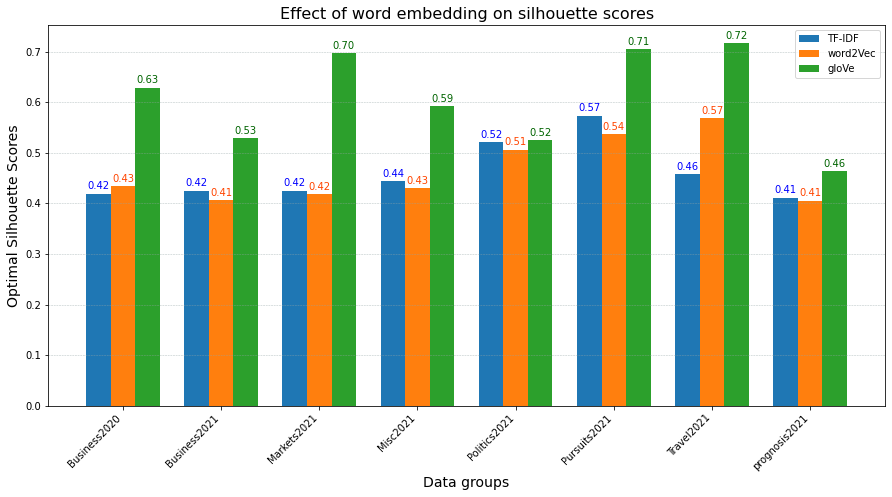
\includegraphics[width=0.7\linewidth]{images/eval/word_embedding.png}
\caption{Effect of using TF-IDF, Word2Vec and GloVe as word embedding model on clustering silhouette scores}
\label{fig:word_embed}
\end{figure}
\vspace{-1em}
As discussed in Section \ref{word_embed_approaches}, in order to cluster the articles, each article's corresponding list of filtered tokens is vectorised. Figure \ref{fig:word_embed}, highlights the effect of the different word embedding techniques, in particular, TF-IDF, Word2Vec and GloVe on the silhouette scores of clusters which are a quantitative measure of of good the clustering is. As indicated by the chart in Figure \ref{fig:word_embed}, using GloVe to vectorise the articles gives a major improvement in the silhouette scores across all the Year-Category input groups, compared to TF-IDF and word2Vec.

\begin{table}[H]
\centering
\renewcommand{\arraystretch}{1.05}
\begin{tabularx}{0.7\textwidth}{X X X} 
\multicolumn{3}{c}{GloVe Percentage Improvement} \\
 \hline
 Data group & TF-IDF & Word2Vec \\
 \hline
 Business 2020 & 50.14\% & 45.02\%  \\ 
 Business 2021 & 24.45\% & 30.13\%  \\
 Markets 2021 & 63.91\% & 66.68\% \\
 Misc 2021 & 33.40\% & 37.81\% \\
 Politics 2021 & 0.76\% & 3.71\% \\
 Pursuits 2021 & 23.06\% & 31.41\%  \\ 
 Travel 2021 & 56.58\% & 26.11\% \\
 Prognosis 2021 & 12.72\% & 14.32\% \\ 
 \hline
 Average & 33.13\% & 31.90\% \\ 
\end{tabularx}
\caption{E-}
\label{table:word_embed}
\end{table}
\vspace{-1em}

Table \ref{table:word_embed} shows the (percentage) improvement in silhouette scores when using GloVe over TF\_TDF and Word2Vec. We see a 33.13\% improvement in clustering (by means of improved silhouette scores) when using GloVe instead of TF-IDF and and 31.90\% improvement when compared to word2Vec. Based on these results, it is evident that using GloVe is the optimal approach for word embedding or token vectorisation for semantic clustering. This is attributed to the fact that most of the silhouette scores are around 0.7 which shows evidence of distinct clusters of articles from which topics can be extracted. When clustering news articles, obtaining a perfect clustering with silhouette score of 1 is very difficult, especially when trying to cluster articles in a particular category within a particular industry. 
% \todonum[inline]{FOR TOPIC MODELLING Do a comparison TABLE for the different sets of allowed postags, Remove adjective noun gives better performance, can show in sil score}

\section{Evaluating topic modelling} \label{s:evaluation_semantic_clustering}

\subsection{Effect of pre-processing on topic modelling} \label{s:preprocess_topic}

\begin{figure}[H]
  \centering
    \begin{minipage}[t]{.49\linewidth}
      \centering
      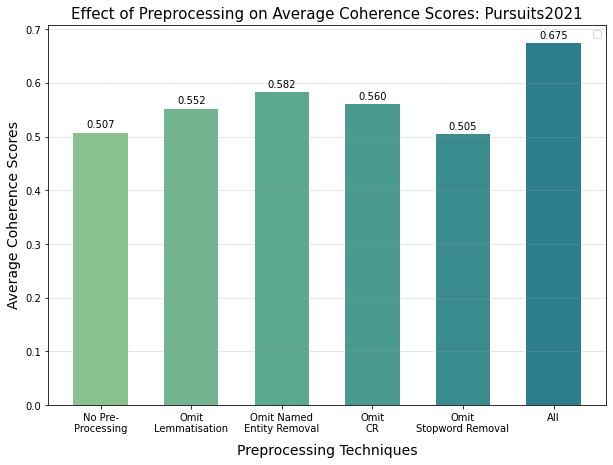
\includegraphics[width=\linewidth]{images/eval/coherence_preprocess.png}
      \caption{-}
      \label{fig:preprocess_topic}
    \end{minipage}
    \begin{minipage}[t]{.49\textwidth}
      \centering
      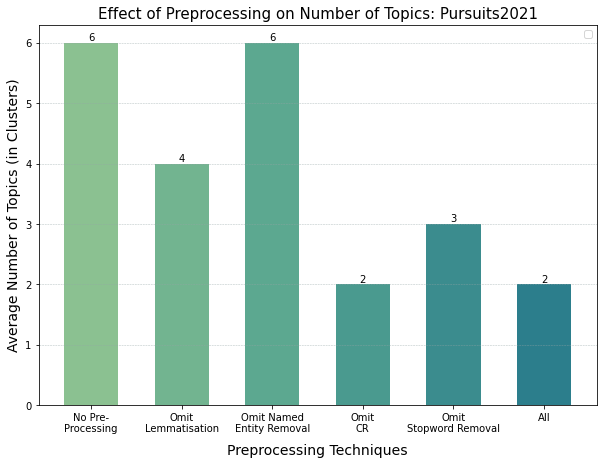
\includegraphics[width=\linewidth]{images/eval/preprocessingTopicNo.png}
      \caption{-}
       \label{fig:pre-processing_topic_no}
    \end{minipage}
  \end{figure}

Section \ref{s:preprocess_clustering} highlights the effect of the different pre-processing techniques on the silhouette scores for semantic clustering. In a similar fashion, Figure \ref{fig:preprocess_topic} depicts the effect of those pre-processing techniques on the topics extracted from all semantic clusters in each Year-Category groups. The topics extracted from each cluster results in a topic coherence score and these are averaged over all clusters to give an average coherence score for a Year-Category group as seen in the figure. In similar trend shown in \ref{s:preprocess_clustering}, the average coherence score of the topics is significantly higher when all the pre-processing techniques are applied which include coreference resolution, named entity removal and stopword removal (represented by the 'All' bar) compared to other approaches. As mentioned previously, coherence score is a metric that assesses the degree of semantic similarity between high-scoring terms in a single topic.

In the case of omitting coreference resolution, the (average) coherence score falls as word tokens such as 'it', 'they', 'those' (essentially, unresolved pronouns) do not contribute to the semantic similarity with other high scoring terms in the corpus. Therefore, resolving these pronouns to their respective nouns, means that the frequency of the nouns increases and they are more likely to contribute to the topics in the corpus. 

The stopwords that are removed in pre-processing contain around 326 words provided as the default stopwords from the SpaCy library for the large English language model \texttt{en-core-wen-lg}. These include words such as \qs{its}, \qs{an}, \qs{the}, \qs{for}, \qs{always}, \qs{here}, \qs{there}, \qs{which}, \qs{moreover} etc. This stopwords list is augmented with a custom list of stopwords which add words such as \qs{told}, \qs{said}, \qs{airline}, \qs{flight} etc. which are specific to the input data. The significance of this custom list is that most articles in the data are quoting an entity usually a person, and therefore words such as  \qs{told}, \qs{said} etc. appear in high frequency but do not provide any relevant information about the content of the articles themselves. Similarly, given the article corpus is specifically for the airline industry, majority articles will have words such as \qs{airline}, \qs{flight} etc. and these are also overarching across majority topics and do not contribute to a distinct topic. The idea is that we do not want the model to fixate on these commonly appearing contentless stopwords and output junk topics, hence why their removing them results in better topic coherence (0.82 denoted by the \qs{All} bar) as seen in \ref{fig:preprocess_topic} compared to when they are retained which results in a lower topic coherence of 0.639. 

Similarly for named entity removal, the aim is to find distinct topics within a cluster that are not dependant on the named entities. For instance, in the input data there are several articles that mention \qs{British Airways} and there are articles cover latent topics such as \qs{pandemic} and \qs{pilot unions}. For arguments sake, let's presume that there is a huge overlap between \qs{pilot unions} and \qs{British Airways}. Retaining named entities in the input corpus would result in \qs{British Airways} the model selecting British Airways as a topic instead of 'pilot unions'. 

\subsection{Effect of POS on topic modelling} \label{s:pos_topic}

\begin{figure}[H]
  \centering
    \begin{minipage}[t]{.49\linewidth}
      \centering
      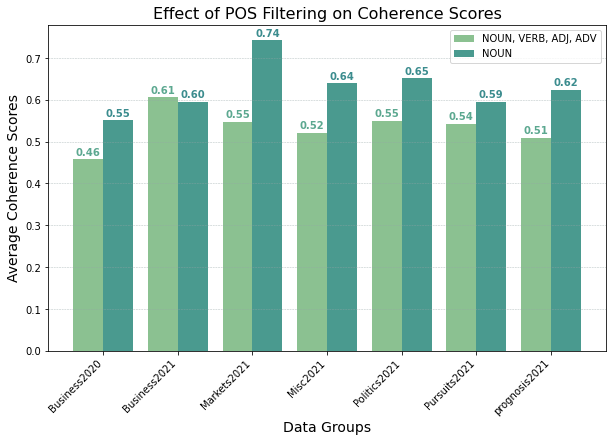
\includegraphics[width=\linewidth]{images/eval/pos_coherence.png}
      \caption{pos}
      \label{fig:pos_topic}
    \end{minipage}
    \begin{minipage}[t]{.49\linewidth}
      \centering
      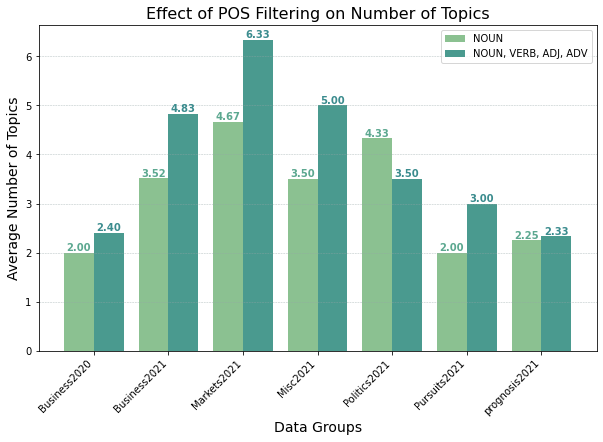
\includegraphics[width=\linewidth]{images/eval/topics_pos.png}
      \caption{-}
       \label{fig:topics_pos}
    \end{minipage}
  \end{figure}


\vspace{-1em}
The filtered tokens list (for each article) that was used to generate the article vectors for clustering, was passed to the LDA model to extract topics from each of the semantic clusters for a Year-Category group. In order to determine the quality of topics extracted, the coherence score measure is used. From~\Cref{fig:pos_topic}, it is apparent that the noun only tokens approach to extract tokens performs better than when noun, adjectives, verbs and adverbs are used as the average coherence scores are generally higher for the former approach. Across all the data groups, we see an average coherence score improvement of 18.2\% with the noun only topic extraction approach.  


% \section{Semantic Triple Extraction Engine}

% \subsection{Entity as Subjects}

\section{Time Efficiency}

\subsection{Comparing Runtimes in Various Environments}
\vspace{-1ex}

\begin{table}[H]
\centering
\renewcommand{\arraystretch}{1.05}
\begin{tabularx}{0.9\textwidth}{X X X X} 
\multicolumn{4}{c}{Time efficiency (in seconds)} \\
 \hline
 {\hsize=.4\hsize\linewidth=\hsize}Data group & {\hsize=.1\hsize\linewidth=\hsize}CPU & {\hsize=.3\hsize\linewidth=\hsize}Multiprocessing CPU & {\hsize=.2\hsize\linewidth=\hsize}GPU \\
 \hline
 Business 2020  & 351.41  & 352.51  & 39.47 \\ 
 Business 2021  & 1713.60 & 1431.80 & 138.47 \\
 Markets 2021   & 839.75  & 1252.64 & 74.18\\
 Misc 2021      & 215.41  & 337.49  & 18.60 \\
 Politics 2021  & 856.42  & 1267.96 & 64.87 \\
 Pursuits 2021  & 178.54  & 377.49  & 15.00 \\ 
 Travel 2021    & 169.52  & 452.80  & 12.92 \\
 Prognosis 2021 & 583.33  & 888.27  & 51.63 \\ 
 \hline
 Total time (s) & 4907.98 & 1920.16 & 414.60 \\ 
 Total time (min) & 81.80  & 32.10 & 6.90\\ 
\end{tabularx}

\caption{E-}
\label{table:cputime}
\end{table}
\vspace{-2ex}
\Cref{table:cputime} shows the different runtimes for the pipeline when running on a CPU, with multiprocessing (on CPU) and GPU. Ideally, the pipeline is meant to be run on the GPU as it results in significant improvement in computation time, with the whole process of running the pipeline for all the input groups from the dataloader taking only 6.9 minutes in comparison. This is 11.8 times faster than running it on the CPU and 4.6 times faster than running it on the CPU with multiprocessing. 

The reason for the high computation time is due to the expensive calls to the AllenNLP models, especially the Fine-Grained NER and SpanBERT Coreference and RoBERTa Sentiment models (see \Cref{s:models}), which unlike spaCy, are not built for production use and therefore not as optimised for time. \hl{However, given that they are state-of-the-art models with high accuracy}, their use is extremely beneficial to the project, motivating the use of multiprocessing and pipelining (see \Cref{fig:sys_arch}) in early stages of development to allow for feasible CPU computation. 

Processes are traditionally constrained to just having access to their own process memory area, but shared memory allows data structures to be shared between processes. In this case, models are stored in shared memory in order to provide centralised access to all running processes and avoid redundant copies of models for each process. This is crucial as the models in question are quite large and therefore, RAM-intensive and so having multiple copies of the models can result in the machine running out memory. 

This allowed running the tool on the 8 different data groups from the dataloader simultaneously. As seen in \Cref{table:cputime}, multiprocessing results in 2.55 times lower computational time compared to running with single process CPU. This is because the idle time is significantly reduced by concurrent processes during the expensive calls for coreference resolution, sentiment analysis and NER. 

\subsection{Effect of different word embedding models on GPU runtime}
\vspace{-1ex}
\begin{table}[H]
\centering
\renewcommand{\arraystretch}{1.05}
\begin{tabularx}{0.9\textwidth}{X X X X} 
\multicolumn{4}{c}{GPU runtime (in seconds)} \\
 \hline
 Data group & TF-IDF & Word2Vec & GloVe \\
 \hline
 Business 2020 & 44.67& 33.82& 39.47 \\ 
 Business 2021 & 256.19 & 130.56 & 138.47 \\
 Markets 2021 & 87.30 & 75.00 & 74.18 \\
 Misc 2021 & 16.67 & 17.92 & 18.60 \\
 Politics 2021 & 60.72 & 71.06 & 64.87 \\
 Pursuits 2021 & 15.00 & 14.38 & 15.00 \\ 
 Travel 2021 & 13.06 & 12.85 & 12.92 \\
 Prognosis 2021 & 53.61 & 59.39 & 51.63 \\ 
 \hline
 Total time (s) & 414.98 & 547.922 & 414.60 \\ 
  Total time (min) & 6.92 & 9.12 & 6.90 \\ 
\end{tabularx}
\caption{Time taken to run the pipeline (on GPU) with different word embedding models}
\label{table:word_embed_time}
\end{table}

\vspace{-3ex}
\Cref{table:word_embed} highlights the time taken for running the pipeline shown in \Cref{fig:sys_arch} on the Tesla T4 GPU for all input data groups (from the dataloader) using different word embedding models.
As established in \Cref{s:word_embeddings}, the Topic Extraction Engine uses \texttt{GloVe} as the word embedding model as it gives a significant improvement in the semantic clustering silhouette scores. In addition to that it also results in more efficient (faster) computation when running the pipeline for all input data with a total runtime of 414.60 seconds, which is 31.15\% lower than using \texttt{Word2Vec}. The difference in runtimes for when using \texttt{TF-IDF} and \texttt{GloVe} is trivial, however, given the 33.13\% improvement in silhouette score of \texttt{GloVe} over \texttt{TF-IDF}, \texttt{GloVe} proves to be the best approach in terms of time efficiency and optimal clustering. 

\section{User Evaluation} \label{s:user_eval}
\hl{In an attempt to gain a greater understanding of the performance of our tool, user testing was conducted with a focus group of 7 people, from DeepSearchLabs to obtain qualitative user evaluation on the utility of the visualisation tool in displaying results from the Topic Extraction Engine and Semantic Triple Extraction Engine.}

% \section*{Dataset Annotation Method, Comparison against state of the art}
% \hl{One form of evaluating our system was to measure the accuracy of topics or relations extracted. Due to the lack of a such as labelled dataset dataset, we initially considered a hand annotated approach to
% match the relations and topics to expected relations and topics for each cluster, in order to have some measure of evaluation.
% However, this would have proven to be very laborious and time-consuming especially but more importantly an unreliable method for empirical evaluation. }


% \hl{When comparing our overall approach to state-of-the-art methodologies in related fields, the
% main limiting factor for this work was the lack of a substantial, annotated dataset specifically tailored to our problem. Due to this, some of the latest technologies and models in natural language processing, which may have improved the capabilities of our tool further, were not able to be applied.}

% \hl{However, through adopting a number of quantitive techniques used for clustering and topic modelling and qualitative analysis for relation extraction, our system is able to produce good results through iterative, empirical modelling and experimentation with different tunings }